% This is samplepaper.tex, a sample chapter demonstrating the
% LLNCS macro package for Springer Computer Science proceedings;
% Version 2.20 of 2017/10/04
%
\documentclass[runningheads]{llncs}
\setcounter{tocdepth}{2}
\makeatletter
\renewcommand*\l@author[2]{}
\renewcommand*\l@title[2]{}
\makeatletter
%
\usepackage{graphicx}
\usepackage{hyperref}
\urlstyle{same}
% Used for displaying a sample figure. If possible, figure files should
% be included in EPS format.
%
% If you use the hyperref package, please uncomment the following line
% to display URLs in blue roman font according to Springer's eBook style:
% \renewcommand\UrlFont{\color{blue}\rmfamily}

\begin{document}
% Global Configs
%
%
\setlength{\tabcolsep}{10pt}
\renewcommand{\arraystretch}{1.5}
%
%
%
\title{Image Recommendation for Wikipedia Articles}
%
%\titlerunning{Abbreviated paper title}
% If the paper title is too long for the running head, you can set
% an abbreviated paper title here
\author{Oleh Onyshchak\inst{1}}
%\authorrunning{F. Author et al.}
% First names are abbreviated in the running head.
% If there are more than two authors, 'et al.' is used.
%
\institute{Ukrainian Catholic University, Lviv, Ukraine\\
\email{o.onyshchak@ucu.edu.ua}\\
\url{https://apps.ucu.edu.ua/en/}}
%
\maketitle              % typeset the header of the contribution
%

\begin{abstract}
Multimodal learning, which is simultaneous learning from different data sources such as audio, text, images; is a rapidly emerging field of Machine Learning. It is also considered to be learning on the next level of abstraction, which will allow us to tackle more complicated problems such as creating cartoons from a plot or speech recognition based on lips movement. 

In this paper, we propose to research whether state-of-the-art techniques of multimodal learning, will solve the problem of recommending the most relevant images for a Wikipedia article. In other words, we need to create a shared text-image representation of an abstract notion which paper describes, so that having only a text description machine would "understand" which images would visualize the same notion accurately. 

\keywords{Multimodal Learning  \and Text-Image Similarity \and Image Recommendation.}
\end{abstract}

\vfill
{
Copyright © 2019 for this paper by its authors. Use permitted under Creative Commons License Attribution 4.0 International (CC BY 4.0).\\
}
\newpage

%
%
%
\tableofcontents
\newpage


\section{Introduction}
Every day we perceive the world around us through multiple cognitive feelings such as sight, smell, hearing, touch, taste. Moreover, our ability to consolidate all the information from different sources into one complete picture helps us comprehensively understand the world.

With a trend to digitizing in the last few decades, more and more information is recorded in different kids of medial such as audio, image, video, text, and 3D modeling. That also created new challenges of efficiently processing a significant amount of recorded information, where we already have significant achievements. However, every type of digital storage only captures some subset of available information. For example, image only captures visual appearance, while  audio - the sound, just as our eyes and ears do. Thus all scientific progress in processing some data carrier is bounded by limitation of what that medium can capture. In other words, to digitally create a notion of a dog, we cannot only have a visual representation. Just as humans, we need to combine all the information streams, which describe the same entity from different perspectives, into one comprehensive representation.

That is the motivation for multimodal representation learning, which aims to combine different types of data into a complete representation of a real-world entity. In that context, the word "modality" refers to a particular way of encoding information. Thus a problem in the domain of e.g., image processing is called unimodal, while a problem in the domain of multiple information encodings e.g., image to caption generation, is called multimodal since it works with both: image and text modalities \cite{ref_survey} 

By having a complete representation of an entity, which was created via multimodal data that captures complementary/supplementary information subsets of an object, we have more comprehensive computational "understanding" of that entity. That will help us to increase the precision of existing data science applications and also extend its limits to more abstract problems such as not only identifying the objects on an image but understanding its value. For example\cite{ref_survey}, early researches on speech recognition showed that by involving visual modality of lips movement on top of sound modality, we get extra information which allows us to increase the quality of voice recognition task, just as it does for humans\cite{ref_human_voice_recognition}

In this project, we are going to research possible approaches for the "Image Recommendation for Wikipedia Articles" problem, which is also part of multimodal representation learning domain. That is, based on the article's text information, we need to recommend images describing the same notion. In other words, we need to create a high-level representation of some entity, described by both text and images. So that later one we can "understand" which image representation of the notion is the best suited for a given text description.

In scope of this project, we are going to explore state-of-the-art techniques of multimodal representation learning and whether they can be applied to solve this problem. We believe this project will be valuable from both a research and an application perspectives.

This report is an official Project Proposal of Master's Thesis, which will formally define the problem, provide rigor overview of state-of-the-art approaches in problem's domain, specify goals of the project, suggest a solution approach and provide a time plan of the thesis.


\section{Problem Motivation}
Wikipedia is the biggest collection of human knowledge containing more than 35 million pages and having nearly 9 billion views per month\footnote{\url{https://stats.wikimedia.org/v2/#/en.wikipedia.org}} And it continually growing, having more than 500 new pages per day\footnote{\url{https://en.wikipedia.org/wiki/Wikipedia:Statistics}}, and all of that only in its English version.

As a part of 2030 strategy, one of the key goals is to break down any barriers for accessing free information\footnote{\url{https://meta.wikimedia.org/wiki/Strategy/Wikimedia_movement/2017/Direction}}. By researching possibilities to automatically recommend images for Wikipedia editors, it will help to get better media enrichment of articles, which in turn will make information easier and faster to comprehend\cite{ref_image_attention}. Also, it would be helpful as automation of time-consuming task to search for and add a proper article visualization. 

In addition to motivation of making Wikipedia better, this work might present some useful insights to development of multimodal learning field. Since this is a 1) purely real-world problem, which might give us interesting insights of how to apply and adjust current academia progress, and also 2) we have a more complicated problem setting of one large article corresponding to a multiple images, instead of more simplified one-to-one correspondas of images and its tags/descriptive sentences.


\section{Problem Formulation}
We are going to research how state-of-the-art multimodal learning techniques performs on a task of recommending images for Wikipedia articles. In other words, having a text with wiki formatting, we need to rank images from Wikimedia Commons database\cite{ref_wiki_commons} by relevance.


\section{Data}
All data is publicly available on Wikipedia. Specifically, we have more than 35 million Wikipedia pages with a fair amount of them enriched with images. We also have Commons image dataset\cite{ref_wiki_commons}, containing more than 55 million images\footnote{\url{https://en.wikipedia.org/wiki/Wikimedia_Commons}}. That is the real-world data, where ultimately the solution should be applied.

But for initial problem research we would only use a reliable subset of above specified data for training. In particular, Wikipedia has a notion of featured articles\footnote{\url{https://en.wikipedia.org/wiki/Wikipedia:Featured_articles}}, which are the best articles with qualitative text and a lot of supporting visualization. In other words, it is a high quality dataset of more than 5000 articles, each of which has multiple associated images, which was manually created. Although, it still requires proper preprocessing and cleaning before using.

Particularly, by text we mean the entire article textual content cleared from Wikipedia formatting along with some extra metadata such as categories or title. Images also collected with additional metadata such as filenames or descriptions. More details can be found on Kaggle\footnote{\url{https://www.kaggle.com/jacksoncrow/wiki-articles-multimodal}}


\section{Related Work}
While during the last decades there was much progress in a field of unimodal representation, research in multimodal learning was limited by simple concatenation of unimodal features\cite{ref_survey_2015}. However, during recent years, the scientific landscape in this domain has been rapidly evolving\cite{ref_survey_baltrusaitis}. One of the triggers for it was the success of deep learning models, which have a powerful representation ability with multiple levels of abstractions. Thus they were also incorporated in multimodal learning. As Guo et al. suggested\cite{ref_survey}, we can divide all the multimodal learning approaches into three categories 1) joint representation, which aims to integrate modality-specific features into some common space 2) coordinated representation, which aims to preserve modality-specific features, while introducing a space to measure multimodal similarities  3) intermediate representation, which aims to encode features of one modal to some intermediate space, from where we later generate features of another modal.

In this chapter, we will cover available techniques to extract features from text and image modalities, overview available solutions in each type of multimodal learning, and then summarise their applicability for our problem.

\begin{figure}
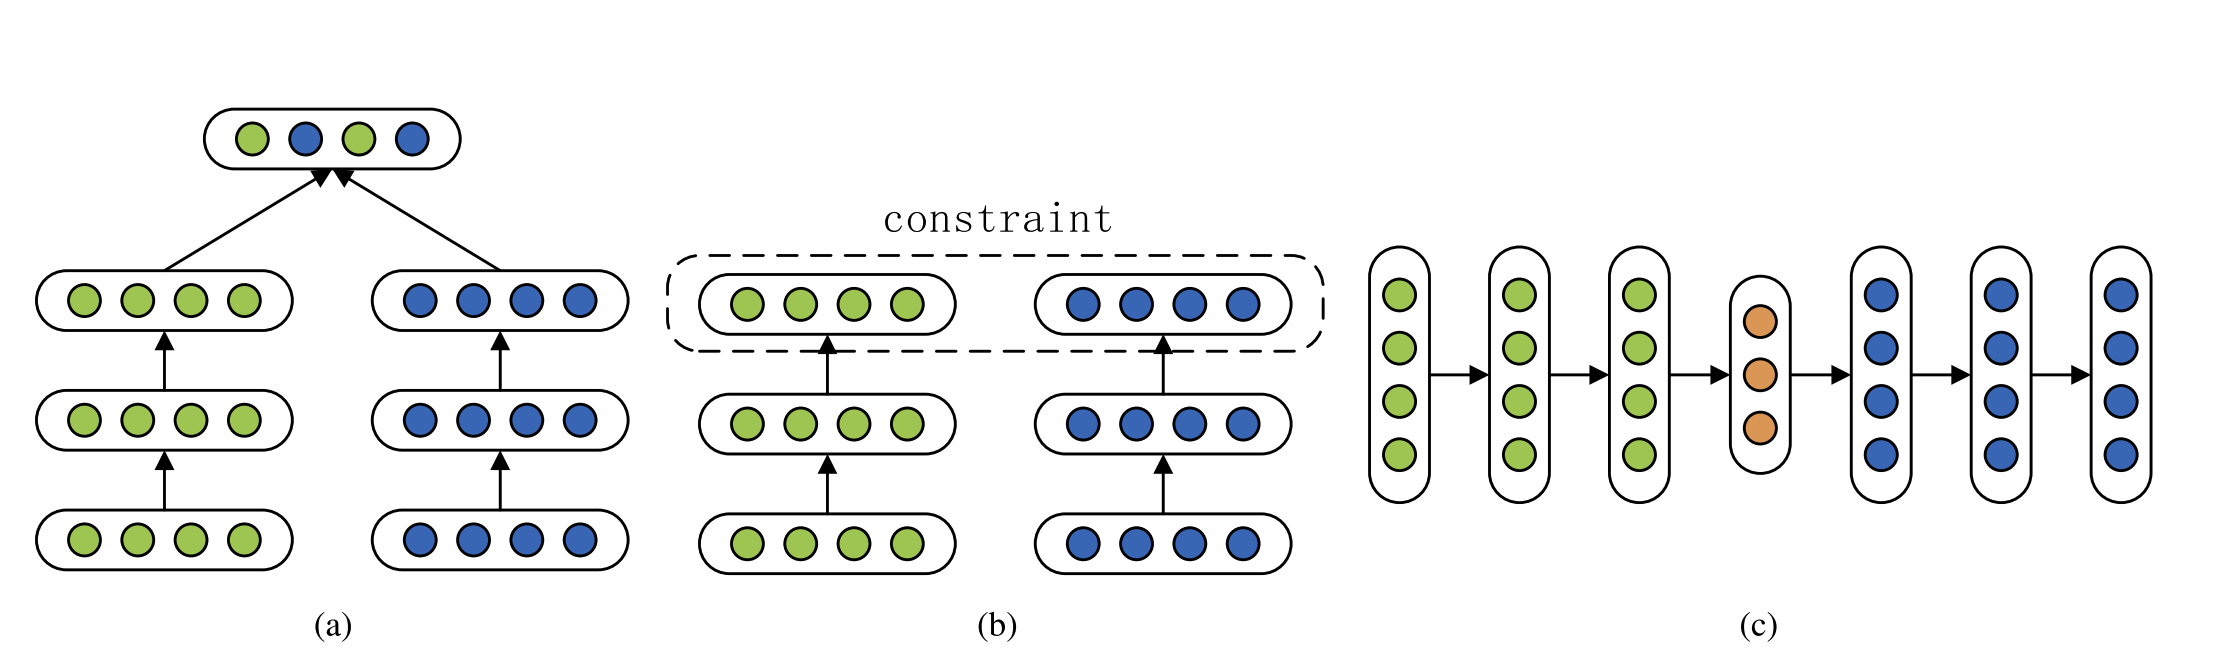
\includegraphics[width=\textwidth]{multimodal_learning_types.png}
\caption{Three types of frameworks about deep multimodal representation. (a) Joint representation aims to learn a shared semantic subspace.(b) Coordinated representation framework learns separated but coordinated representations for each modality under some constraints.
(c) intermediate representation framework translates one modality into another and keep their semantics consistent.\cite{ref_survey}} \label{fig1}
\end{figure}

\subsection{Unimodal Representation}
\subsubsection{Image}
The most popular model used in feature extraction from images are different types of Convolutional Neural Network(CNN), such as AlexNet\cite{ref_AlexNet}, VGGNet\cite{ref_VGGNet} and ResNet\cite{ref_ResNet}. When working with big datasets, it is preferable to use pre-trained version of chosen CNN. This field has tremendous development in recent years, and thus currently we already have well-defined solution for most problems.

\subsubsection{Text}
A popular way to extract features from the text is to encode it to vector, as is done in word2vec\cite{ref_word2vec} or Glove\cite{ref_glove} algorithms. They map words into one-hot encoded vector space of language vocabulary. Although, the common problem with those approaches is when some words are not present in vocabulary or out-of-vocabulary error. However, there are also a variety of solutions to this problem, such as character embeddings\cite{ref_char_embeddings}. 

An alternative and more powerful tool for dealing with text is recurrent neural network(RNN)\cite{ref_rnn}, which is more context-aware and can make better encoding of the n-th word, knowing what was already in a sentence. One of the most successful realizations of RNN is long short-term memory(LSTM)\cite{ref_lstm}.

\subsection{Joint Representation}
The main idea of joint representation is to integrate multimodal features into a single input, which we then process as some artificial unimodal input with well-known machine learning techniques. More formally, it aims to project unimodal representations into a shared semantic subspace, where the multimodal features can be fused\cite{ref_survey_baltrusaitis},  as shown in Figure \ref{fig1}(a). Up until recently, that was the primary technique in multimodal learning, where shared features were fused by concatenating them together. However, now,  the most popular choice is to use a distinct hidden layer, where modality-specific features will be combined into a single output vector.

This approach was historically the first one and is still commonly applicable in video classification\cite{ref_video_class}, event detection\cite{ref_event_detection} and visual question answering\cite{ref_visual_question_answ}. However, its main disadvantage is neglecting the fact that different modalities have not only supplementary information, that is which show the same notion from different perspectives, but also complementary information, where one modality captures the information which another cannot. For example, lips movement and audio of a speech are mostly supplementary sources, while images of some bird and audio of it singing are mostly supplementary sources. Because of that, much information gets lost in that shared space. 
% TODO: explain why in examples above one is supplementary and another complemetary

Although it has advantages of being a simple method and producing modality-invariant common space of features, it cannot be used to infer the separated representations for each modality\cite{ref_survey}. Thus methods from this category are not applicable to our problem

\subsection{Intermediate Representation}
Intermediate Representation models aim to encode features of one modality to some intermediate space, from which later features of another modality can be generated(or decoded), as shown on Figure \ref{fig1}(c). To prevent the intermediate space from being related only to a source modality, during encoder-decoder training we maximize, e.g., the likelihood of target sentence given source image, so that error function employs the error of decoding. Subsequently, the generated intermediate representation tends to capture the shared semantics from both modalities\cite{ref_survey}. 

Some interesting application of that model was proposed by Mor et al.\cite{ref_music_decoder}, where algorithm encodes a musical track into intermediate space, which then will be decoded by multiple decoders into a space of some specific instrument. In other words, encoder extracts instrument-invariant generic musical features, which then each decoder transforms into features of its target instrument.

The general advantage of such approach is that it is one of the best ways to generate new features in a target domain. Thus this technique is used in Image Caption\cite{ref_image_caption}, Video Description\cite{ref_video_description}, and Text to Image\cite{ref_text2image} generations. The disadvantages of that model are that 1) it can only encode one modality, 2) complexity of designing a feature generator should be taken into account\cite{ref_survey} and 3) intermediate space also extracts only shared subspace from two modalities. Moreover, because we need to query existing information rather than generate one, those methods are also not suitable for our problem solution.

\subsection{Coordinated Representation}
The last type of multimodal learning is a coordinated representation. Instead of learning from a joint representation, it learns from modal-specific representations separately but with a shared constraint, which is some loss function identifying cross-modal similarity/correlation. Since different modalities hold unique information about an object, that approach operates with all available knowledge. A visual explanation can be seen in Figure \ref{fig1}(b). Regarding constraint function, a commonly used option is cross-modal similarity functions, where learning objective is to preserve both inter-modality and intra-modality similarity structure. In other words, it would force cross-modal distance for elements with the same semantics be as small as possible, while with dissimilar - as big as possible. 

% TODO: specify what specifically function S can be and how it works
The cross-modal ranking is a widely used constrain, where the loss function is defined in the following way
\begin{equation} \label{eq_rank_loss}
\sum_i \sum_{t^-} max(0, \alpha - S(i, t) + S(i, t^-)) + \sum_t \sum_{i^-} max(0, \alpha - S(t, i) + S(t, i^-))
\end{equation}
where (i,t) is a matching image-text pair, $\alpha$ is margin, S is a similarity function, $i^-$ is mismatching pair to $t$ and vise versa. Frome et al.\cite{ref_devise} used a combination of dot-product similarity and margin rank loss to learn a visual-semantic embedding model(DeViSE) for visual recognition\cite{ref_survey}. DeViSE trains deep networks for both image and text features, and then adjust features based on above mentioned ranked loss, though in more simplified form.

Alternatively to cross-modal ranking, another widely used constraint is Euclid distance, which is also used for ensuring that similarity structure for both intra-modality and inter-modality is preserved. That is, for inter-modality, we map text and image features into low-dimensional space, where we can calculate the distance between feature vectors. The idea here is to ensure that inter-modality features of the same semantics are as close as possible\cite{ref_pan}. While for intra-modality, we want to preserve the similarity between neighborhood items, that is:
$$ d(m_i, m_j) + m < d(m_i, m_k), \forall m_j \in N(m_i), \forall m_k \notin N(m_i),$$
where $m$ is data point of any modality, $m_i$ point of interest, N(m) - denotes neighborhood of m\cite{ref_wang}.
% TODO: what is m specifically in a formula? Correct it!

So, Coordinated Representation preserves all modality-specific information. It also explicitly compares features from different modalities, thus having data from one, we can identify the closest data point from another modality. Because of those properties, it is used for cross-modal retrieval\cite{ref_wang}, retrieval-based visual description\cite{ref_socher}, and transfer knowledge across modalities\cite{ref_pan}. Thus it can be applied for our problem of Image Recommendation for articles, and we will proceed with those methods.


\section{Solution Approach}
After rigor overview of related work, Coordinated Representation techniques were identified as the most prominent direction for our problem. Coordinated Representation approach aims to exploit modality-specific features fully, thus we train each feature modality separately.
% TODO: for our solution? (not problem)

To make the system learn right features in each modality, we map all of them into space where inter-modality similarity can be evaluated but also preserving the intra-modality similarity structure\cite{ref_cross_modal_hash}\cite{ref_devise}\cite{ref_kiros}. Then we identify loss function, by enforcing ranking function (\ref{eq_rank_loss}) in that space to return high values for mismatches modality pairs and small otherwise. That would be a loss function, which each modality-specific model will be minimizing, thus empowering modality-specific feature learning. You can see visualisation of this idea on Figure \ref{fig2}.

\begin{figure}
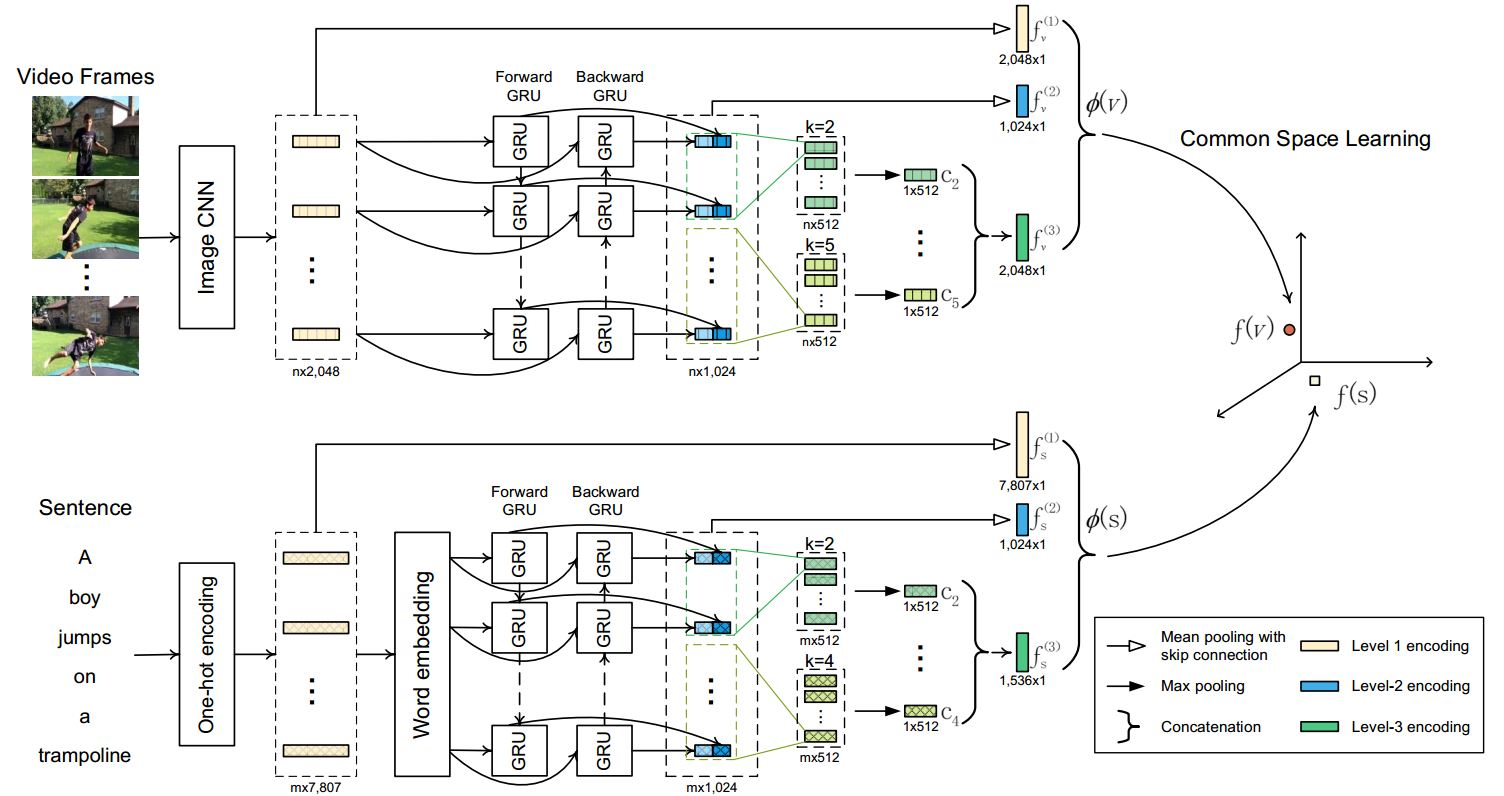
\includegraphics[width=\textwidth]{dual_encoding.jpg}
\caption{Example of Coordinated Representation learning pipeline\cite{ref_dual_encoding}} \label{fig2}
\end{figure}

We will focus on integrating recent Word2VisualVec\cite{ref_w2vv} and dual encoding\cite{ref_dual_encoding} models to our more broader and more realistic problem settings. They showed impressive results but were evaluated on more narrow problem. More specifically, they were working with Flickr dataset\cite{ref_flickr} where one image corresponds to 5 descriptive sentences. In our settings we have one article corresponding to multiple images, where all of them having additional metadata such as category, name, description.

This paper is supported by Github repository\footnote{\url{https://github.com/OlehOnyshchak/WikiImageRecommendation}} with all experiments

\section{Methodology}
\subsection{Methodological Approach}
The hypothesis under test is: "it is possible to implement a model to recommend relevant Commons\cite{ref_wiki_commons} images for a specific Wikipedia article using multimodal learning techniques" and implies Quantitative research. It is aiming to discover whether state-of-the-art techniques of multimodal representation learning can solve this specific problem for Wikipedia with not worse precision. 

\subsection{Methods of Data Collection}
Existing Wikipedia data will be used to conduct the research. More specifically, we will use a collection of featured articles\footnote{\url{https://en.wikipedia.org/wiki/Wikipedia:Featured_articles}}, where each page went through thorough manual review procedure by the Wikipedia community and represent the best Wikipedia can offer. Thus it is theoretically the best possible quality for machine learning algorithms.

\subsection{Methods of Analysis}
We will select candidate algorithms by analyzing recent literature surveys of a corresponding domain, and choosing the most prominent state-of-the-art approaches described there. We will also check the most cited approaches to solve a similar problem. In that way, we can ensure that all state-of-the-art methods existing in that field would be reviewed and then the most applicable would be adequately tested.

\subsection{Evaluation}
Since we have a labeled dataset, classical evaluation metrics would be applied here. Currently, the most appropriate approach is rank-based performance metric \cite{ref_evalmetric} P@K (K=1,5,10), where P is the percentage of articles for which corresponding images are found within the top $K * N_{images}$ images, where $N_{images}$ is the number of images of this article.

When scaling up on real-world image dataset size, evaluation metrics will require additional improvements such as merging visually similar images from top-ranked matches, although it is out of the scope of testing our hypothesis.


\section{Goals}
The goal of the project is to research whether it is possible to implement a system, which would recommend relevant Commons\cite{ref_wiki_commons} images for a specific Wikipedia article. Thus we are planning to investigate the scientific landscape in that area and provide report whether it can solve our specific problem of image recommendation with Wikipedia dataset. We do not expect to create a complete end-to-end solution but rather investigate a path towards it is feasible.

\section{Time Plan}
\begin{center}
 \begin{tabular}{| l | l |} 
 \hline
 Date & Milestone \\
 \hline
 10 Sep 2019 & Kick Start \\
 \hline
 16 Sep 2019 & Project Proposal's Abstract Submission \\
 \hline
 30 Sep 2019 & Project Proposal Submission \\  
 \hline
 1 Nov 2019 & Start of Implementation \\  
 \hline
 15 Nov 2019 & Finalise Approach and Solution \\  
 \hline
 1 Dec 2019 & Start of Evaluation \\  
 \hline
 10 Dec 2019 & Finalise Evaluation Planning \\  
 \hline
 23 Dec 2019 & Finalise Implementation \\  
 \hline
 27 Dec 2019 & Finalise Evaluation \\ 
 \hline
 31 Dec 2019 & Finalise Review of Related Work \\ 
 \hline
 8 Jan 2020 & Thesis Final Submission \\
 \hline
\end{tabular}
\end{center}

%
% ---- Bibliography ----
%
% BibTeX users should specify bibliography style 'splncs04'.
% References will then be sorted and formatted in the correct style.
%
% \bibliographystyle{splncs04}
% \bibliography{mybibliography}
%
\begin{thebibliography}{8}
\bibitem{ref_survey}
Guo, Wenzhong, Jianwen Wang, and Shiping Wang. "Deep Multimodal Representation Learning: A Survey." IEEE Access 7 (2019): 63373-63394.

\bibitem{ref_human_voice_recognition}
McGurk, Harry, and John MacDonald. "Hearing lips and seeing voices." Nature 264.5588 (1976): 746.

\bibitem{ref_survey_baltrusaitis}
Baltrušaitis, Tadas, Chaitanya Ahuja, and Louis-Philippe Morency. "Multimodal machine learning: A survey and taxonomy." IEEE Transactions on Pattern Analysis and Machine Intelligence 41.2 (2018): 423-443.

\bibitem{ref_survey_2015}
D'mello, Sidney K., and Jacqueline Kory. "A review and meta-analysis of multimodal affect detection systems." ACM Computing Surveys (CSUR) 47.3 (2015): 43.

\bibitem{ref_w2vv}
Dong, Jianfeng, Xirong Li, and Cees GM Snoek. "Predicting visual features from text for image and video caption retrieval." IEEE Transactions on Multimedia 20.12 (2018): 3377-3388.

\bibitem{ref_dual_encoding}
Dong, Jianfeng, et al. "Dual Encoding for Zero-Example Video Retrieval." Proceedings of the IEEE Conference on Computer Vision and Pattern Recognition. 2019.

\bibitem{ref_flickr}
Plummer, Bryan A., et al. "Flickr30k entities: Collecting region-to-phrase correspondences for richer image-to-sentence models." Proceedings of the IEEE international conference on computer vision. 2015.

\bibitem{ref_AlexNet}
Krizhevsky, Alex, Ilya Sutskever, and Geoffrey E. Hinton. "Imagenet classification with deep convolutional neural networks." Advances in neural information processing systems. 2012.

\bibitem{ref_VGGNet}
Simonyan, Karen, and Andrew Zisserman. "Very deep convolutional networks for large-scale image recognition." arXiv preprint arXiv:1409.1556 (2014).

\bibitem{ref_ResNet}
He, Kaiming, et al. "Deep residual learning for image recognition." Proceedings of the IEEE conference on computer vision and pattern recognition. 2016.

\bibitem{ref_image_attention}
Vogel, Douglas Rudy, Gary W. Dickson, and John A. Lehman. Persuasion and the role of visual presentation support: The UM/3M study. Minneapolis: Management Information Systems Research Center, School of Management, University of Minnesota, 1986.

\bibitem{ref_cross_modal_hash}
Jiang, Qing-Yuan, and Wu-Jun Li. "Deep cross-modal hashing." Proceedings of the IEEE conference on computer vision and pattern recognition. 2017.

\bibitem{ref_word2vec}
Mikolov, Tomas, et al. "Efficient estimation of word representations in vector space." arXiv preprint arXiv:1301.3781 (2013).

\bibitem{ref_glove}
Pennington, Jeffrey, Richard Socher, and Christopher Manning. "Glove: Global vectors for word representation." Proceedings of the 2014 conference on empirical methods in natural language processing (EMNLP). 2014.

\bibitem{ref_char_embeddings}
Kim, Yoon, et al. "Character-aware neural language models." Thirtieth AAAI Conference on Artificial Intelligence. 2016.

\bibitem{ref_rnn}
Elman, Jeffrey L. "Finding structure in time." Cognitive science 14.2 (1990): 179-211.

\bibitem{ref_lstm}
Hochreiter, Sepp, and Jürgen Schmidhuber. "Long short-term memory." Neural computation 9.8 (1997): 1735-1780.

\bibitem{ref_video_class}
Jiang, Yu-Gang, et al. "Exploiting feature and class relationships in video categorization with regularized deep neural networks." IEEE transactions on pattern analysis and machine intelligence 40.2 (2017): 352-364.

\bibitem{ref_wiki_commons}
Wikimedia Commons, Wikimedia\\
\url{https://commons.wikimedia.org/wiki/Main_Page}


\bibitem{ref_event_detection}
Habibian, Amirhossein, Thomas Mensink, and Cees GM Snoek. "Video2vec embeddings recognize events when examples are scarce." IEEE transactions on pattern analysis and machine intelligence 39.10 (2016): 2089-2103.

\bibitem{ref_visual_question_answ}
Fukui, Akira, et al. "Multimodal compact bilinear pooling for visual question answering and visual grounding." arXiv preprint arXiv:1606.01847 (2016).

\bibitem{ref_music_decoder}
Mor, Noam, et al. "A universal music translation network." arXiv preprint arXiv:1805.07848 (2018).

\bibitem{ref_image_caption}
Vinyals, Oriol, et al. "Show and tell: A neural image caption generator." Proceedings of the IEEE conference on computer vision and pattern recognition. 2015.

\bibitem{ref_video_description}
Venugopalan, Subhashini, et al. "Translating videos to natural language using deep recurrent neural networks." arXiv preprint arXiv:1412.4729 (2014).

\bibitem{ref_text2image}
Reed, Scott, et al. "Generative adversarial text to image synthesis." arXiv preprint arXiv:1605.05396 (2016).

\bibitem{ref_evalmetric}
Ma, Lin, et al. "Multimodal convolutional neural networks for matching image and sentence." Proceedings of the IEEE international conference on computer vision. 2015.

\bibitem{ref_devise}
Frome, Andrea, et al. "Devise: A deep visual-semantic embedding model." Advances in neural information processing systems. 2013.

\bibitem{ref_kiros}
Kiros, Ryan, Ruslan Salakhutdinov, and Richard S. Zemel. "Unifying visual-semantic embeddings with multimodal neural language models." arXiv preprint arXiv:1411.2539 (2014).

\bibitem{ref_socher}
Socher, Richard, et al. "Grounded compositional semantics for finding and describing images with sentences." Transactions of the Association for Computational Linguistics 2 (2014): 207-218.

\bibitem{ref_pan}
Pan, Yingwei, et al. "Jointly modeling embedding and translation to bridge video and language." Proceedings of the IEEE conference on computer vision and pattern recognition. 2016.

\bibitem{ref_wang}
Wang, Liwei, Yin Li, and Svetlana Lazebnik. "Learning deep structure-preserving image-text embeddings." Proceedings of the IEEE conference on computer vision and pattern recognition. 2016.

\end{thebibliography}

\end{document}
